\documentclass{article}
\usepackage{graphicx} % Required for inserting images
\usepackage[utf8]{inputenc}
\usepackage[T1]{fontenc} 
\usepackage[polish]{babel}
\usepackage{hyperref}
\usepackage{graphicx}

\title{\textbf{Specyfikacja funkcjonalna programu dzielącego graf}}
\author{Adam Domański, Oliwier Osiński}
\date{30.04.2025}

\begin{document}

\maketitle

\section*{Link do repozytorium:}
\url{https://github.com/t0q1/JIMP2_graph_C/tree/main}

\section*{Cel projektu}

Celem projektu jest stworzenie programu dzielącego graf w języku C. Program ma podzielić graf określoną liczbę razy, przy jak najmniejszej liczbie usuniętych krawędzi. Różnica w liczbie wierzchołków w nowo utworzonych grafach nie może się różnić o więcej niż podany przez użytkownika margines procentowy. Wszystkie parametry mają być przyjmowane z linii poleceń. Program ma wypisywać otrzymany graf w trybie tekstowym lub binarnym w zależności od preferencji użytkownika.

\section*{Argumenty wywołania programu}
Do prawidłowego uruchomienia programu należy podać następujące argumenty:
\begin{itemize}
    \item ścieżka pliku wejściowego: ścieżka do pliku, który zawiera tekstową interpretację grafu;

    \item liczba podzieleń grafu (N): dodatnia liczba całkowita, której domyślna wartość wynosi 1;

    \item margines różnicy procentowej między powstałymi grafami (M): nieujemna liczba całkowita, której domyślna wartość wynosi 10 (wartości interpretowane w procentach);

    \item ścieżka pliku wyjściowego: ścieżkę do pliku, w którym zostanie zapisany graf po dokonaniu podziałów
    
\end{itemize}

\section*{Plik wejściowy}
Do prawidłowego dokonania podziału grafu potrzebne będą informacje o grafie, który ma zostać podzielony. Dane te mają być zapisane w formacie tekstowym w pliku txt.\\

\textbf{Plik z grafem wejściowym składa się z następujących linii:}

\begin{itemize}
  \item Maksymalna liczba węzłów w wierszu.
  \item Indeksy węzłów w poszczególnych wierszach.
  \item Wskaźniki na pierwsze indeksy węzłów w liście wierszy.
  \item Grupy węzłów połączone przy pomocy krawędzi.
  \item Wskaźniki na pierwsze węzły w poszczególnych grupach.
\end{itemize}
\textbf{Przykład grafu w pliku wejściowym:}\\
\texttt{3\\0;2;1;0\\0;2;3\\1;3;4;4;2\\0;3;5}

\section*{Dane wyjściowe}
Wyniki operacji programu mogą zostać wyświetlone lub zapisane na dwa różne sposoby.
\begin{enumerate}
\item W domyślnym trybie tekstowym najpierw w pierwszej linii zwracana jest wartość pomyślnie podzielonych grafów, a następnie podzielone grafy w identycznym formacie jak w pliku wejściowym.

\item W trybie binarnym, gdzie ma być zwracane tylko grafy. Tryb ten nie ma z góry określonego formatu.
\end{enumerate}

Warto zaznaczyć, że w zależności od podanych flag, program może jednocześnie wyświetlić wynik w terminalu, jak i zapisać go do pliku.\\

\textbf{Program przyjmuje następujące flagi:}
\begin{itemize}
\item -h - flaga wyświetla instrukcje obsługi programu

\item -o plik.out - flaga przyjmuje argument w postaci ścieżki do pliku, w którym ma zostać zapisany wynik operacji

\item -t - flaga powoduje wyświetlenie wyniku w terminalu

\item -b - flaga zmienia sposób wyświetlania wyniku z tekstowego na binarny
\end{itemize}

\newpage

\section*{\textbf{Specyfikacja implementacyjna programu dzielącego graf}}


\section*{Struktura plików}
Opisywany program składa się z następujących katalogów i plików:
\begin{itemize}
    \item Makefile - plik wykonywalny kompilujący i uruchamiający różne testowe scenariusze programu;
    \item bin - katalog zawierający skompilowany program o nazwie "graf";
    \item include - katalog zawierający pliki nagłówkowe;
    \item src - katalog zawierający pliki źródłowe c;
    \item tests - katalog zawierający testowe pliki wejściowe opisujące grafy
\end{itemize}

\section*{Argumenty wywołania}
Do poprawnego uruchomienia programu niezbędne jest podanie jednego obowiązkowego argumentu. Opcjonalnie można dodać dwa dodatkowe argumenty zmieniające parametry programu.
\begin{enumerate}
    \item \textbf{plik.in} - ścieżka do pliku, w którym zapisany jest graf przeznaczony do podziału.\\\\
    W przypadku, gdy podany plik nie istnieje, program zróci błąd o treści: Blad: Nie udalo sie otworzyc pliku wejsciowego o podanej sciezkce. Przerywam dzialanie.\ i zakończy działanie.\\\\
    Natomiast, gdy dane przedstawiające graf są niepoprawne, program zwróci błąd o treści: "Blad: Dane w pliku przedstawiajace graf sa niepoprawne. Przerywam dzialanie."\ i zakończy działanie.
    
    \item \textbf{N} (opcjonalny) -  dodatnia liczba całkowita podzieleń grafu na podgrafy, której wartość domyślna wynosi \textbf{1}.\\\\
    W przypadku, gdy nie poda się wartości liczbowej, program zwróci błąd o treści: "Blad: Liczba podzieleń grafu została niepoprawnie zdefiniowana. Przerywam działanie."\ i zakończy działanie.\\\\
    Natomiast, gdy podana liczba, będzie niedodatnie lub zmiennoprzecinkowa, to program zwróci błąd o treści: "Blad: Liczba podzieleń grafu musi być większa bądź równa 1. Przerywam działanie."\ i zakończy działanie.

    \item \textbf{M} (opcjonalny) - nie ujemna liczba całkowita nie przekraczająca wartości 100, liczba przedstawia graniczną wartość procentową, pod którą musi się zmieścić różnica wierzchołków podzielonych podgrafów, jej domyślna wartość wynosi \textbf{10}.\\\\
    W przypadku, gdy nie poda się wartości liczbowej, program zwróci błąd o treści: "Blad: Liczba marginesu różnicy procentowej została niepoprawnie zdefiniowana. Przerywam działanie."\ i zakończy działanie.\\\\
    Natomiast, gdy podana liczba, będzie ujemna lub zmiennoprzecinkowa, to program zwróci błąd o treści: "Blad: Liczba marginesu różnicy procentowej między wierzchołkami powstałych grafów musi znajdować się w przedziale [0-100]. Przerywam działanie."\ i zakończy działanie.
\end{enumerate}


Przykłady użycia argumentów podczas wywoływania programu znajdują się w sekcji \textbf{Uruchomienie programu}.

\section*{Flagi}
Program przyjmuje następujące flagi:
\begin{itemize}
    \item \textbf{-h} - flaga wyświetlająca informacje o argumentach programu oraz dostępne flagi wraz z ich opisami.
    \item \textbf{-o plik.out} - flaga przyjmująca jako argument ścieżkę do pliku, do którego ma zostać zapisany wynik końcowy programu. Domyślna wartość argumentu flagi to \textbf{"wynik.txt"}.

    \item \textbf{-b} - flaga zmienia tryb wyświetlania wyniku z domyślnie tekstowego na binarny.

    \item \textbf{-t} - flaga sprawiająca, że wynik końcowy programu zostanie wypisany w terminalu. Można łączyć z flagą -b, wtedy w terminalu zostanie wyświetlony wynik binarny.
\end{itemize}

Przykłady użycia flag podczas wywoływania programu znajdują się w sekcji \textbf{Uruchomienie programu}.

\section*{Uruchomienie programu}
Do kompilacji programu należy użyć komendy \textbf{make} w terminalu lub od razu wybrać wcześniej przygotowany scenariusz testowy, wpisując \textbf{make \{nazwa\_testu\}} o których więcej w sekcji \textbf{Testy}.
\\

Aby uruchomić program należy w teminalu wywołać plik wykonywalny znajdujący się w katalogu bin: \textbf{/bin/graf}, a następnie podać odpowiednie argumenty, o których mowa była w sekcjach \textbf{Argumenty wywołania} oraz \textbf{Flagi}.\\

Przykład wywołania programu wczytującego graf z pliku /tests/graf.csrrg, wypisującego wynik w trybie tekstowym w terminalu oraz do pliku podzial.txt:
\textbf{./bin/graf /tests/graf.csrrg 2 20 -o podzial.txt -t}\\

Przykład wywołania programu wczytującego graf z pliku /tests/graf2.csrrg, wypisującego wynik w trybie binarnym w terminalu:\\
\textbf{./bin/graf /tests/graf2.csrrg -t -b}

\section*{Format wyjściowy}
Program zawsze zapisuje końcowy wynik w pliku, który został podany w odpowiedniej fladze podczas wywoływania (domyślnie "wynik.txt").\\

Na wynik końcowy w trybie tekstowym (domyślny) składa się:
\begin{itemize}
    \item Liczba udanych podziałów grafu w pierwszej linijce.

    \item Następnie graf w takim samym formacie co w pliku wejściowym.
\end{itemize}

W przypadku trybu binarnego, podawany jest jedynie sam graf. Sposób zapisania grafu w postaci binarnej przedstawia sekcja \textbf{Plik binarny}.

\section*{Plik binarny}
W trybie binarnym każda liczba reprezentowana jest binarnie na 32 bitach. Znak \textbf{\textbackslash n} jest reprezantowany przez ciąg 32 jedynek, natomiast znak \textbf{;} przez ciąg 31 jedynek i zera.\\

\textbf{Przykładowo:}

\begin{itemize}
  \item Liczba 5 jest reprezentowana przez 00000000000000000000000000000101
  \item Znak \textbf{\textbackslash n} przez 11111111111111111111111111111111
  \item Znak \textbf{;} przez 11111111111111111111111111111110

  Przykład:
  graf w formie tekstowej: 5\textbackslash n0;2;4;1;3;0;1;2;3\textbackslash n0;3;5;9\textbackslash n0;1;4;7;5;5;8;6;8;7\textbackslash n0;2;5;7
  zapisa w postaci binarnej:\\
  00000000000000000000000000000101
  11111111111111111111111111111111
  00000000000000000000000000000000
  11111111111111111111111111111110
  00000000000000000000000000000010
  11111111111111111111111111111110
  00000000000000000000000000000100
  11111111111111111111111111111110
  00000000000000000000000000000001
  11111111111111111111111111111110
  00000000000000000000000000000011
  11111111111111111111111111111110
  00000000000000000000000000000000
  11111111111111111111111111111110
  00000000000000000000000000000001
  11111111111111111111111111111110
  00000000000000000000000000000010
  11111111111111111111111111111110
  00000000000000000000000000000011
  11111111111111111111111111111111
  00000000000000000000000000000000
  11111111111111111111111111111110
  00000000000000000000000000000011
  11111111111111111111111111111110
  00000000000000000000000000000101
  11111111111111111111111111111110
  00000000000000000000000000001001
  11111111111111111111111111111111
  00000000000000000000000000000000
  11111111111111111111111111111110
  00000000000000000000000000000001
  11111111111111111111111111111110
  00000000000000000000000000000100
  11111111111111111111111111111110
  00000000000000000000000000000111
  11111111111111111111111111111110
  00000000000000000000000000000101
  11111111111111111111111111111110
  00000000000000000000000000000101
  11111111111111111111111111111110
  00000000000000000000000000001000
  11111111111111111111111111111110
  00000000000000000000000000000110
  11111111111111111111111111111110
  00000000000000000000000000001000
  11111111111111111111111111111110
  00000000000000000000000000000111
  11111111111111111111111111111111
  00000000000000000000000000000000
  11111111111111111111111111111110
  00000000000000000000000000000010
  11111111111111111111111111111110
  00000000000000000000000000000101
  11111111111111111111111111111110
  00000000000000000000000000000111
\end{itemize}

Zapis grafu w formacie binarnym nie zawiera spacji, tylko stały ciąg zer i jedynek. Powyższy przykład zawiera spacje dla łatwiejszej wizualizacji.

\section*{Pliki źródłowe}
W katalogu src znajdują się następujące pliki:
\begin{itemize}
    \item \textbf{main.c} - plik, w którym obsługiwane są argumenty i flagi wywołujące program oraz inicjalizuje podział grafu.

    \item \textbf{grapf.c} - plik zawierający funkcje do obsługi struktury grafu oraz funkcje odpowiedzialne za faktyczny podział grafu.

    \item \textbf{file\_graph.c} - plik zawierający funkcje odpowiedzialne za odczyt grafu z pliku, jak i jego zapis do pliku.

    \item \textbf{getopt.c} - plik zawierający funkcje do poprawnego i bezbłędnego odczytu argumentów oraz flag wywoływanego programu.
    
\end{itemize}

\newpage

\section*{Struktury}
\textbf{Struktura grafu:}\\

\begin{figure}[ht]
  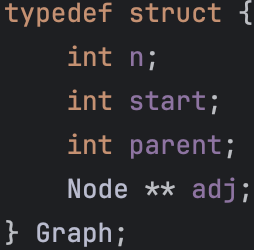
\includegraphics[]{img/graph.png}
\end{figure}
gdzie:
\begin{itemize}
    \item n - liczba wierzchołków grafu
    \item start oraz parent - zmienne potrzebne do podziału grafu
    \item adj - "lista" wierzchołków grafu
\end{itemize}

\textbf{Struktura wierzchołka:}\\
\begin{figure}[ht]
  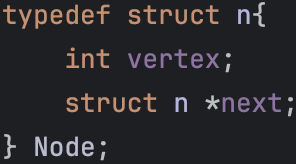
\includegraphics[]{img/node.png}
\end{figure}\\
gdzie:
\begin{itemize}
    \item vertex - etykieta wierzchołka
    \item next - wskaźnik do następnego wierzchołka
\end{itemize}

\newpage

\section*{Funkcja podziału grafu}
Użyty w naszych programie algorytm do podziału grafu jest uproszczoną wersją algorytmu Kerninghana-Lina. \\
W pierwszym kroku wierzchołki są reprezentowane w tablicy intów o długości ilości wierzchołków w grafie, etykieta węzła odpowiada indeksowi w tej tablicy. Do tablicy przypisywane są po równo wartości (0 i 1), wartości te będą reprezentować na koniec dwa grafy, jeden z wierzchołkami o wartościach 0 i drugi z wierzchołkami o wartościach 1. Następnie przy pomocy pętli, algorytm przechodzi kolejno wszystkie wierzchołki w tablicy i sprawdza czy przeniesienie danego wierzchołka (zmiana wartość na przeciwną) do drugiej części zmniejsza liczbę przecięć. Warto zaznaczyć, że wierzchołek jest przenoszony tylko wtedy gdy nie zaburzy równowagi dwóch części. Następnie z powstałej tablicy składającej się z 0 i 1, są tworzone dwa grafy. W przypadku gdy powstałe grafy spełniają warunek różnicy liczby wierzchołków, to pierwotny dzielony graf w tablicy grafów jest podmieniany na pierwszy nowo powstały graf, a drugi powstały graf jest dodawany na koniec tablicy grafów. W przypadku gdy nie spełniają tego warunku, indeks wskazujący na obecny graf w tablicy grafów jest zwiększany o jeden i proces podziału zaczyna się od początku dla kolejnego grafu w kolejce. Po zakończeniu wszyskich podziałów grafów, wszyskie grafy z tablicy grafów zostają scalone w jeden duży graf, który ma tyle samo wierzchołków co graf wczytywany z pliku wejściowego. Ze względu na parametry start i parent w strukturze grafu, każdy graf zna pierwotne wartości etykiet z wczytywanego grafu. Następnie funkcja zwróci liczbę udanych podziałów grafów i cały proces dobiegnie do końca. 

\end{document}
